\chapter{Results}
\label{chapter:results}

\section{Test infrastructure description}
\label{section:testprogram}

In order to create a test program for the above methods we have to determine the requirements for such a program. Since we are interested in determining allocation sizes and allocation points, the test program has to provide a sufficiently diverse combination of these. Our program also has to be deterministic so that we test the methods against the same sequence of allocations. The number of allocations has to be sufficiently high so that the overhead of monitoring becomes noticeable.

In order to keep things simple and focus on the techniques and not on what the program does, the main task of our test program is to allocate a linked list whose nodes contain pointers to malloc-allocated memory whose size is controllable. In other words, we have a list of memory regions allocated with malloc. The linked list's nodes are also heap allocated and since there is one node for each allocation we can say that the number of actual allocations is twice that we give as input to the program. We are also interested in being able to control the depth at which the allocations are made, in order to be able to determine the overhead of stack tracing as the stack increases in size.

Most programs have memory usage patterns containing a mix of allocations and deallocations. Having a test program which contains just allocations would not be representative for the majority of these patterns. Thus, we introduce the capability of deallocating some of the allocated memory through a simple counter which triggers the release of a previously allocated memory region. In the end, the core loop of the test program has the following pseudocode, where capitalized variables are given by the user:

\begin{lstlisting}[label=pseudotest, caption=Test program core loop]
for NR_ITERATIONS do
	for size = START_SIZE, size < END_SIZE, size += STEP_SIZE
		call function such that allocation of size bytes is made at depth DEPTH in the call stack
		if DEALLOCATION_COUNTER reached zero then free previous allocation and reset DEALLOCATION_COUNTER
\end{lstlisting}

First, we want to determine the overhead of determining the size of each allocation and compare it with the overhead of periodically sampling and traversing data structures. These are the two major approaches we can take in determining the amount of memory a specific program occupies. The final goal of allocation size monitoring is to be able to determine memory consumption on a per-module basis. Total memory consumption is not an issue, as this can be determined through other mechanisms which are usually provided by the operating system. The main problem is to have more fine grained memory reporting. For now, however, the test program is only interested in determining the total size of all the allocations we do. At this point, we are only trying to determine the overhead of obtaining the allocation data so we ignore the overhead of its utilization in finely grained memory reporting. In order to do this, we test the following scenarios:
\begin{enumerate}
\item \textit{On-demand data structure traversal} - go through the linked list and use malloc\_usable\_size on each node and the memory region it points to
\item \textit{On-demand counter based monitoring} - have the linked list hold a counter representing the total allocated size, which is updated whenever a node is added or removed; access the counter whenever the total allocated size is required
\item \textit{GCC provided malloc hooks} - use these to insert own code which updates a global variable containing total allocated bytes
\item \textit{GCC aided call replacement} - write own allocation routines which do the counting and then call the existing ones to actually do the allocation
\item \textit{Manually defined malloc-wrappers} - use the preprocessor or just write own routines which do the counting and then call the allocation routines
\item \textit{Dynamically linked library containing malloc implementations} - very similar to the call replacement except it is not GCC dependent
\end{enumerate}

Second, to determine the overhead of obtaining stack traces, we test the following:
\begin{enumerate}
\item \textit{GCC provided malloc hooks} - contain a parameter which gives the return address found on the stack
\item \textit{Global stack object} - manually keep a copy of the stack on the heap and access that copy whenever we want to a stack trace
\item \textit{Manual stack walk} - use low-level platform information about the stack's format to perform a manual walk
\item \textit{External library (libunwind)} - an existing library which abstracts away all the details of the stack and provides a simple way of accessing it
\end{enumerate}

Running the basic program under Valgrind with the "none" tool performs approximately 5 times worse than without Valgrind. To be more specific, the average runtime of the Valgrind run, doing 120000 allocations of 128 bytes is around 146 milliseconds while the basic run has an average runtime of 27 milliseconds. This performance ratio holds for other number of allocations and sizes. The "none" tool does no work at all so it is a good way to measure the overhead of Valgrind's code translation overhead. Since this overhead is significantly higher than the above mentioned approaches, we will not take Valgrind into consideration for determining allocation sizes and allocation points.

\section{Allocation size overhead results}
\label{section:allocsz}

One problem when comparing the two main methods of obtaining allocation sizes is to make sure that the results we obtain are the same so that the work can be fairly compared. Taking a closer look at these methods we observe that on-demand data structure traversal has a simple yet very important advantage over overloading the allocation routines: easy association between the data structures and their size. Our simple scenario has us incrementing a global variable which keeps track of the total amount of allocated memory so we don't need such an association. The initial purpose was however to provide a more granular memory reporting solution. To make the comparison more fair, code that walks the entire stack manually has been inserted in the overloaded allocation routines. This information would then theoretically be used to provide an accurate location of where the allocation was made.

\begin{figure}[htb]
\centering
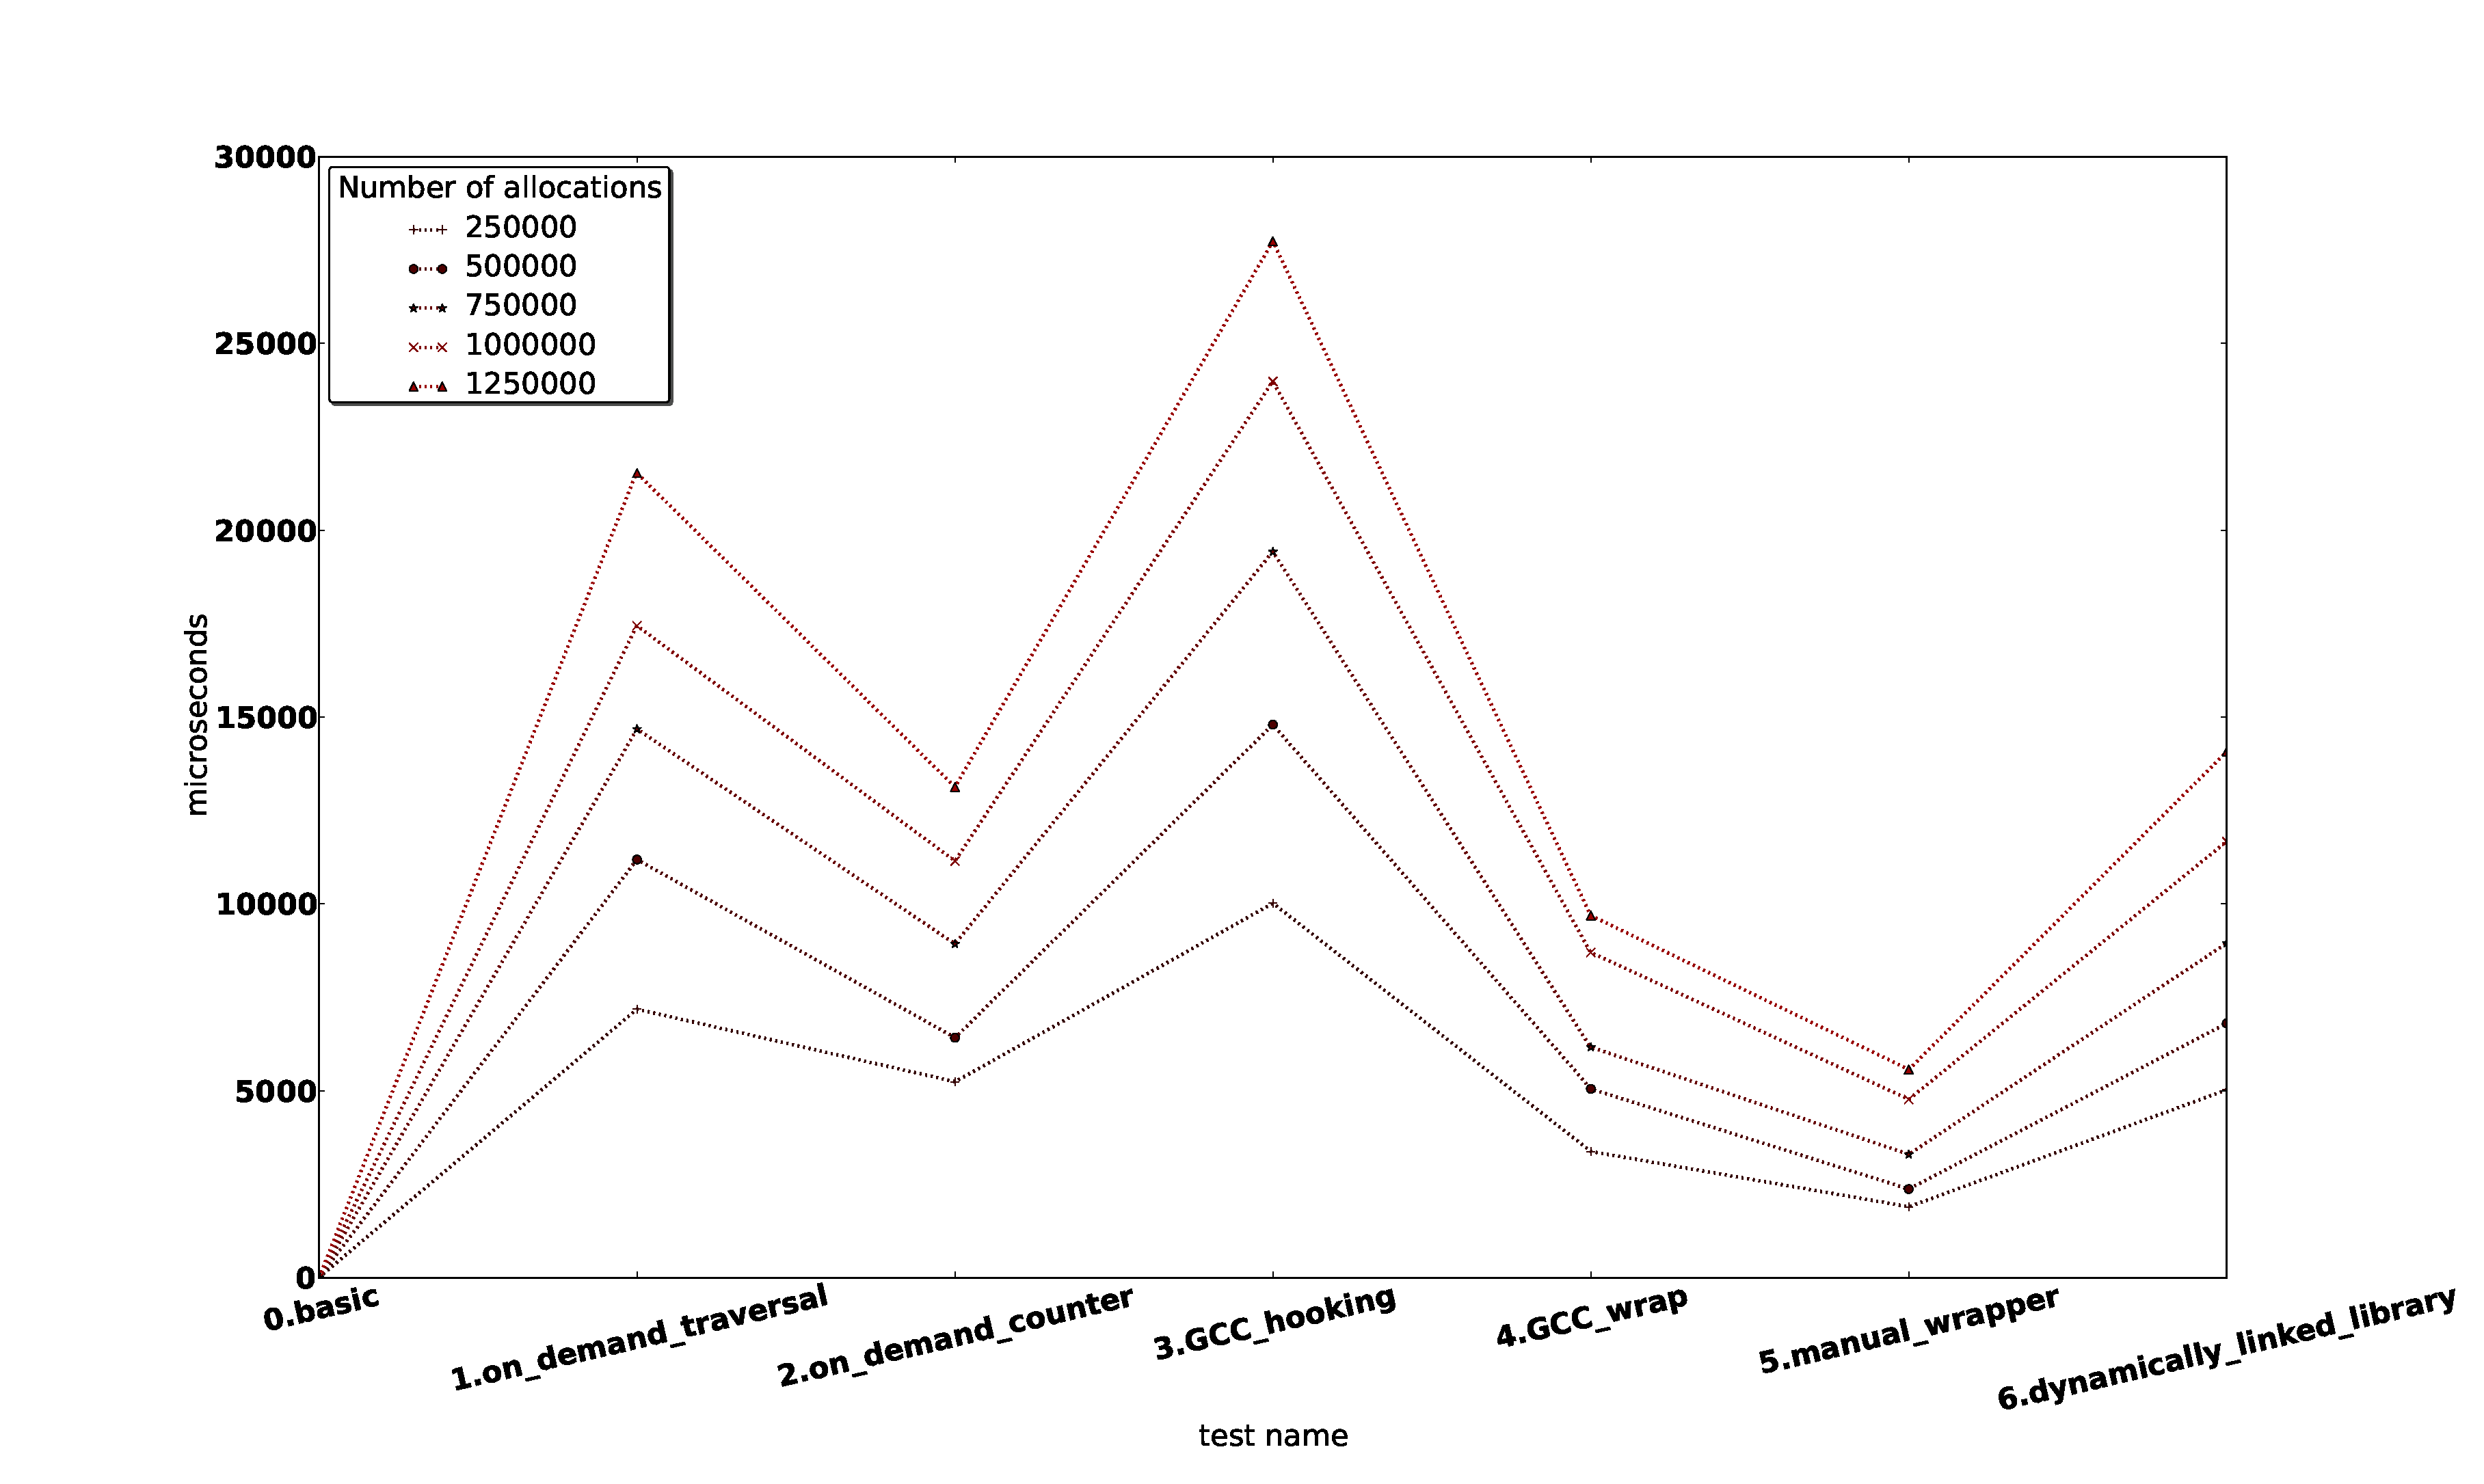
\includegraphics[width=1.0\textwidth]{src/img/allocationsizewithoutlogging}
\caption{Allocation size time overhead compared to the basic scenario when no logging is done}
\label{fig:allocszwithoutlog}
\end{figure}

\begin{figure}[htb]
\centering
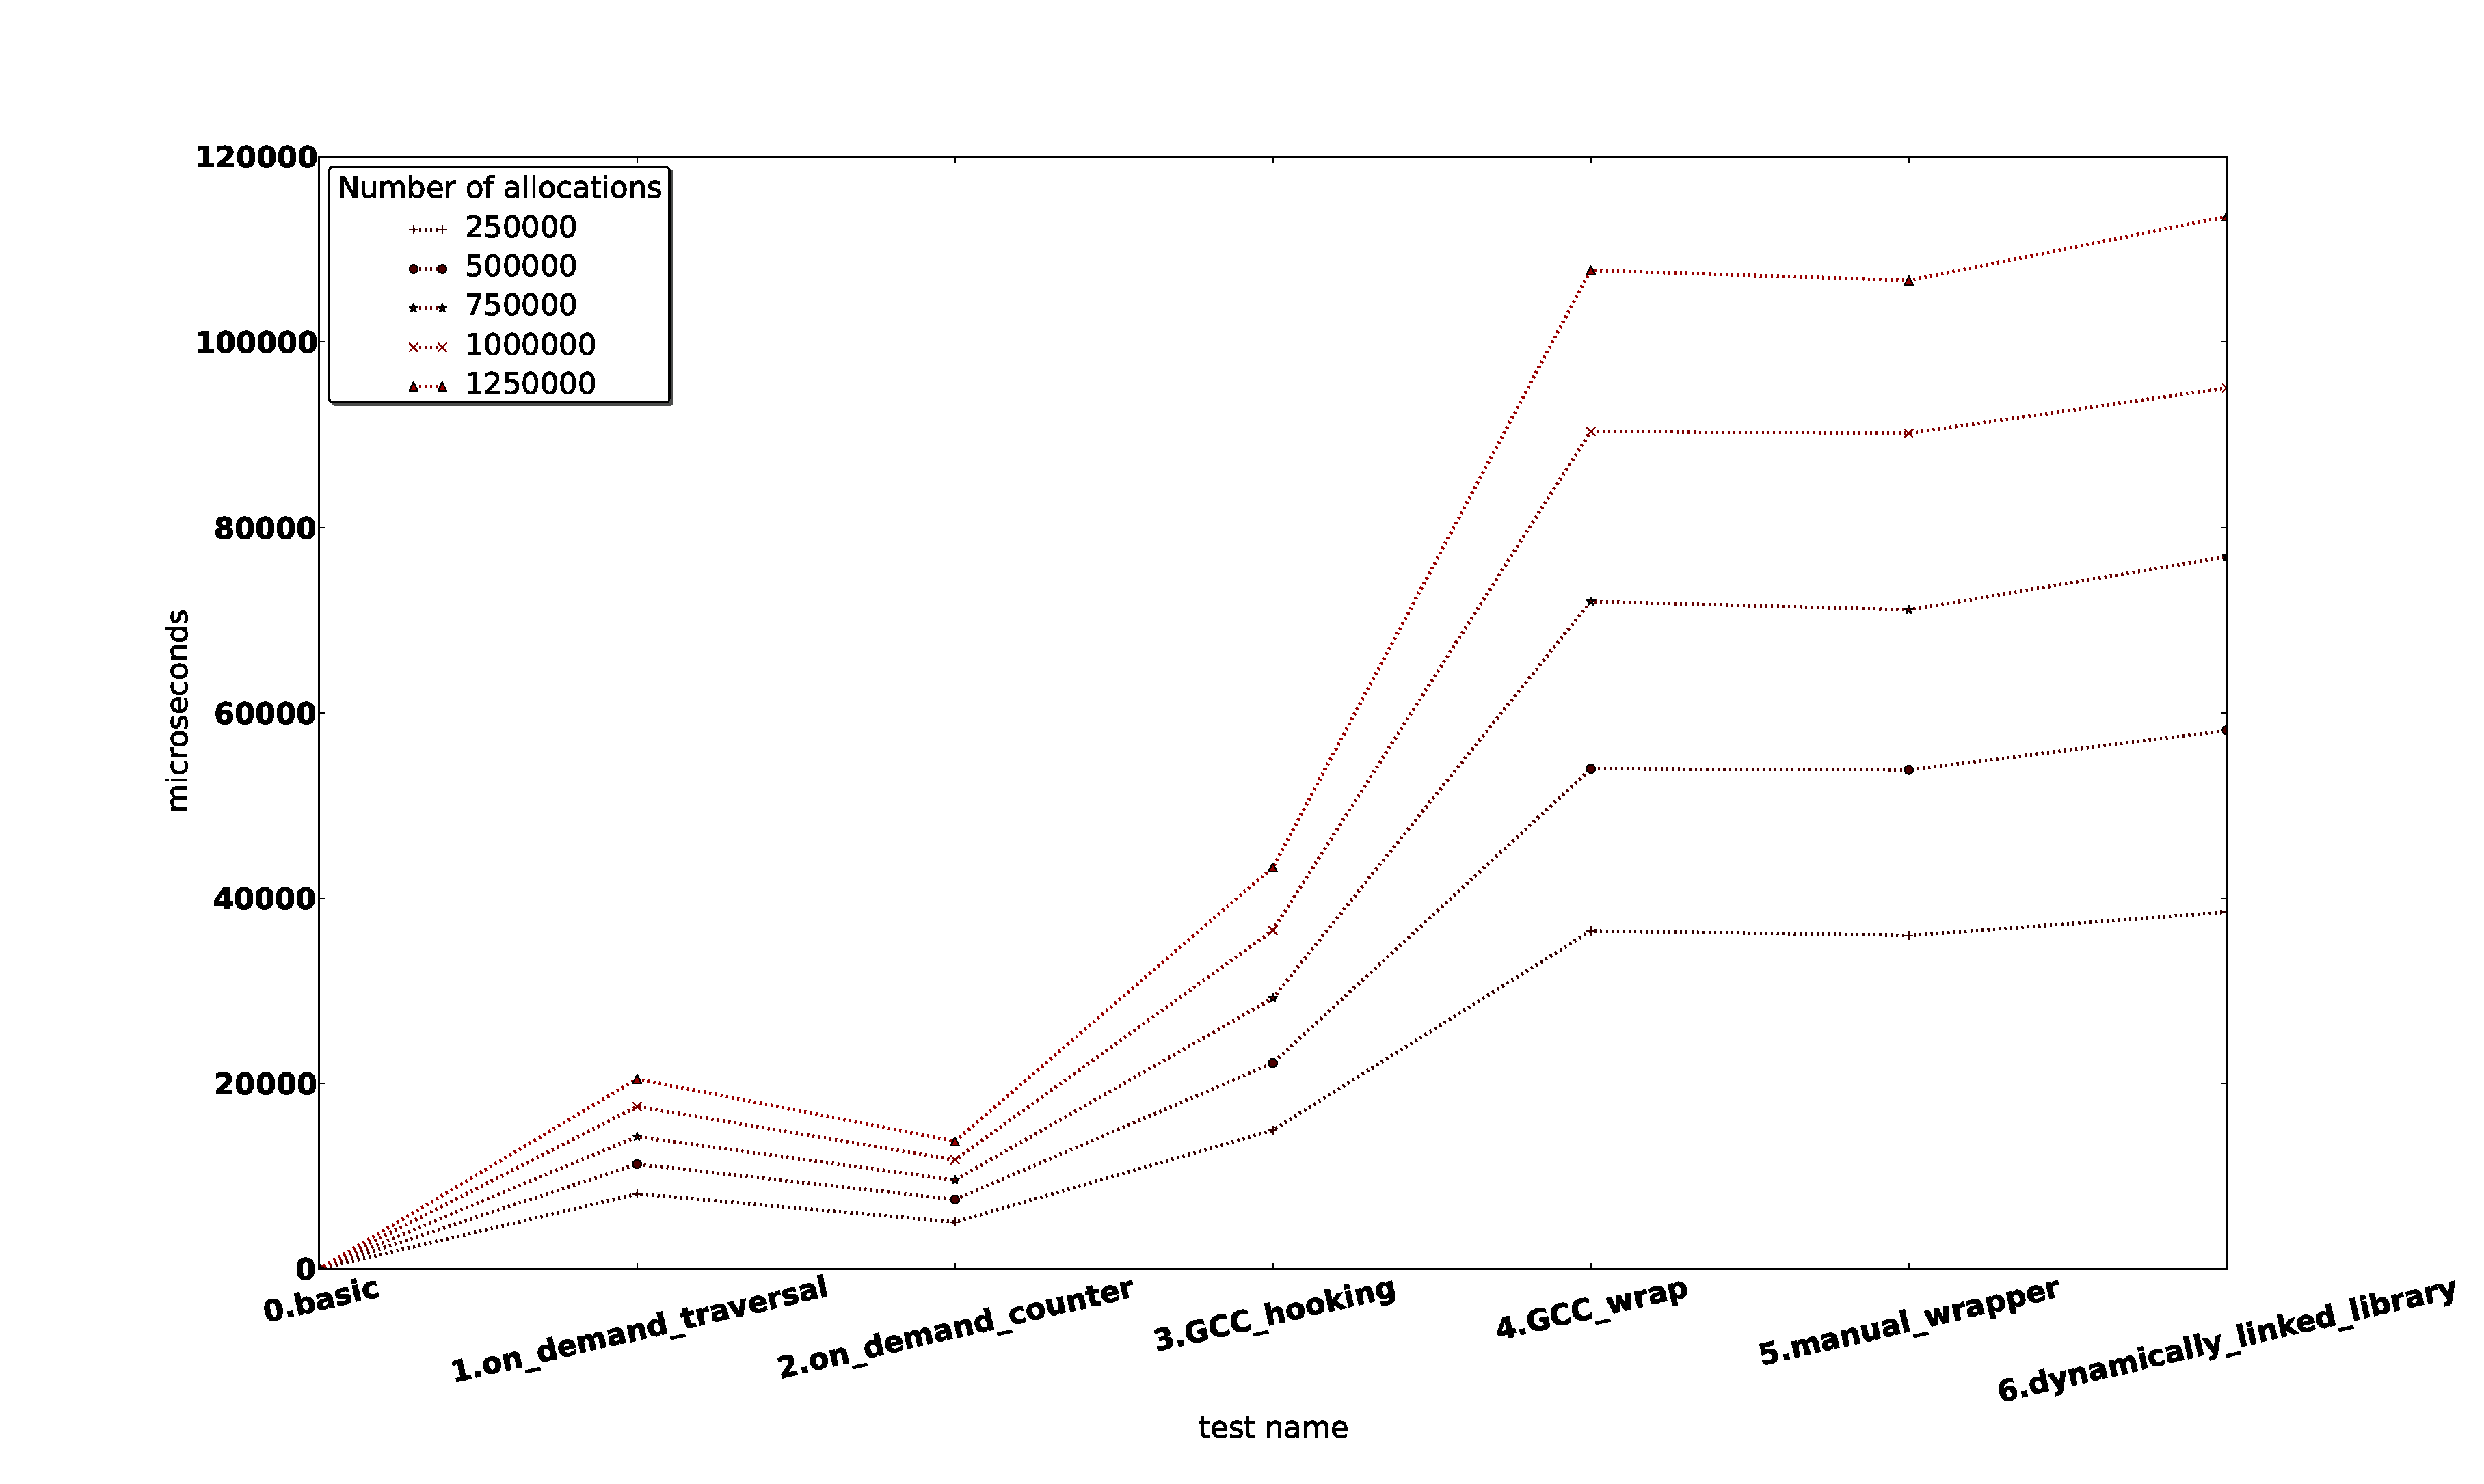
\includegraphics[scale=0.5, width=\textwidth]{src/img/allocationsizewithlogging}
\caption{Allocation size time overhead compared to the basic scenario when logging is done}
\label{fig:allocszwithlog}
\end{figure}

In figure \ref{fig:allocszwithoutlog} we can see that the overhead of overloading is lower than the traversal's when we only increment/decrement the global variable. This is explained by the fact that the traversal involves sequential access through each list element which in turn generates extra page faults and cache misses. The overhead of these additional memory accesses is thus higher at this point than the work done inside the overloaded allocation routines. In figure \ref{fig:allocszwithlog} however, we can see that this is no longer true when we add the stack walking. The conclusion to be drawn from this is that the actual mechanisms used to obtain the allocation size information are not the ones inducing the overhead but rather the work performed inside these mechanisms. Since a lot of work needs to be done in the overloaded allocation routines in order to correctly identify the place where the allocation was made, they do perform worse than the traversal techniques.

* Perhaps a graph with exact Valgrind overhead related to number of allocations

\section{Allocation point overhead results}
\label{section:allocpt}

In figure \ref{fig:allocpoint} the time overhead of the allocation point determination is shown. While it may seem that the malloc hooks provide the best solution, it has to be mentioned that they only provide the caller of the malloc routine which makes them useless for practical purposes. For the hooks to provide the same amount of information as the other methods, they would have to be augmented with a similar stack walking routine which would put them on the same overhead level as the manual walking method.

Comparing the global stack object with manual stack walking we can see that the former appears to be significantly better. There is one small catch related to the global stack object and that is its behaviour in a multithreaded environment. Multiple buffers are required, one for each thread. Additional code has to be added to check which thread has called the current function, in order to determine in which buffer the trace will be placed. Another disadvantage is that every method has to be augmented at entry and exit points with calls to the object's logging method. This could be done before compile time, by an automatic script. That being said, calls are expensive so inlining might be a solution, at the expense of increased code size.

Finally, using libunwind has such a high overhead that when the results get added to the graph, the other three methods' plot points degenerate into a line. It has thus been omitted from the graph but the method does have its merits. Such a library represents the most portable way of implementing allocation point tracing. Being able to ignore all the low-level details and use a common interface for all of them represents a huge benefit which might make this method suitable if the performance hit is acceptable to the application.

\begin{figure}[htb]
\centering
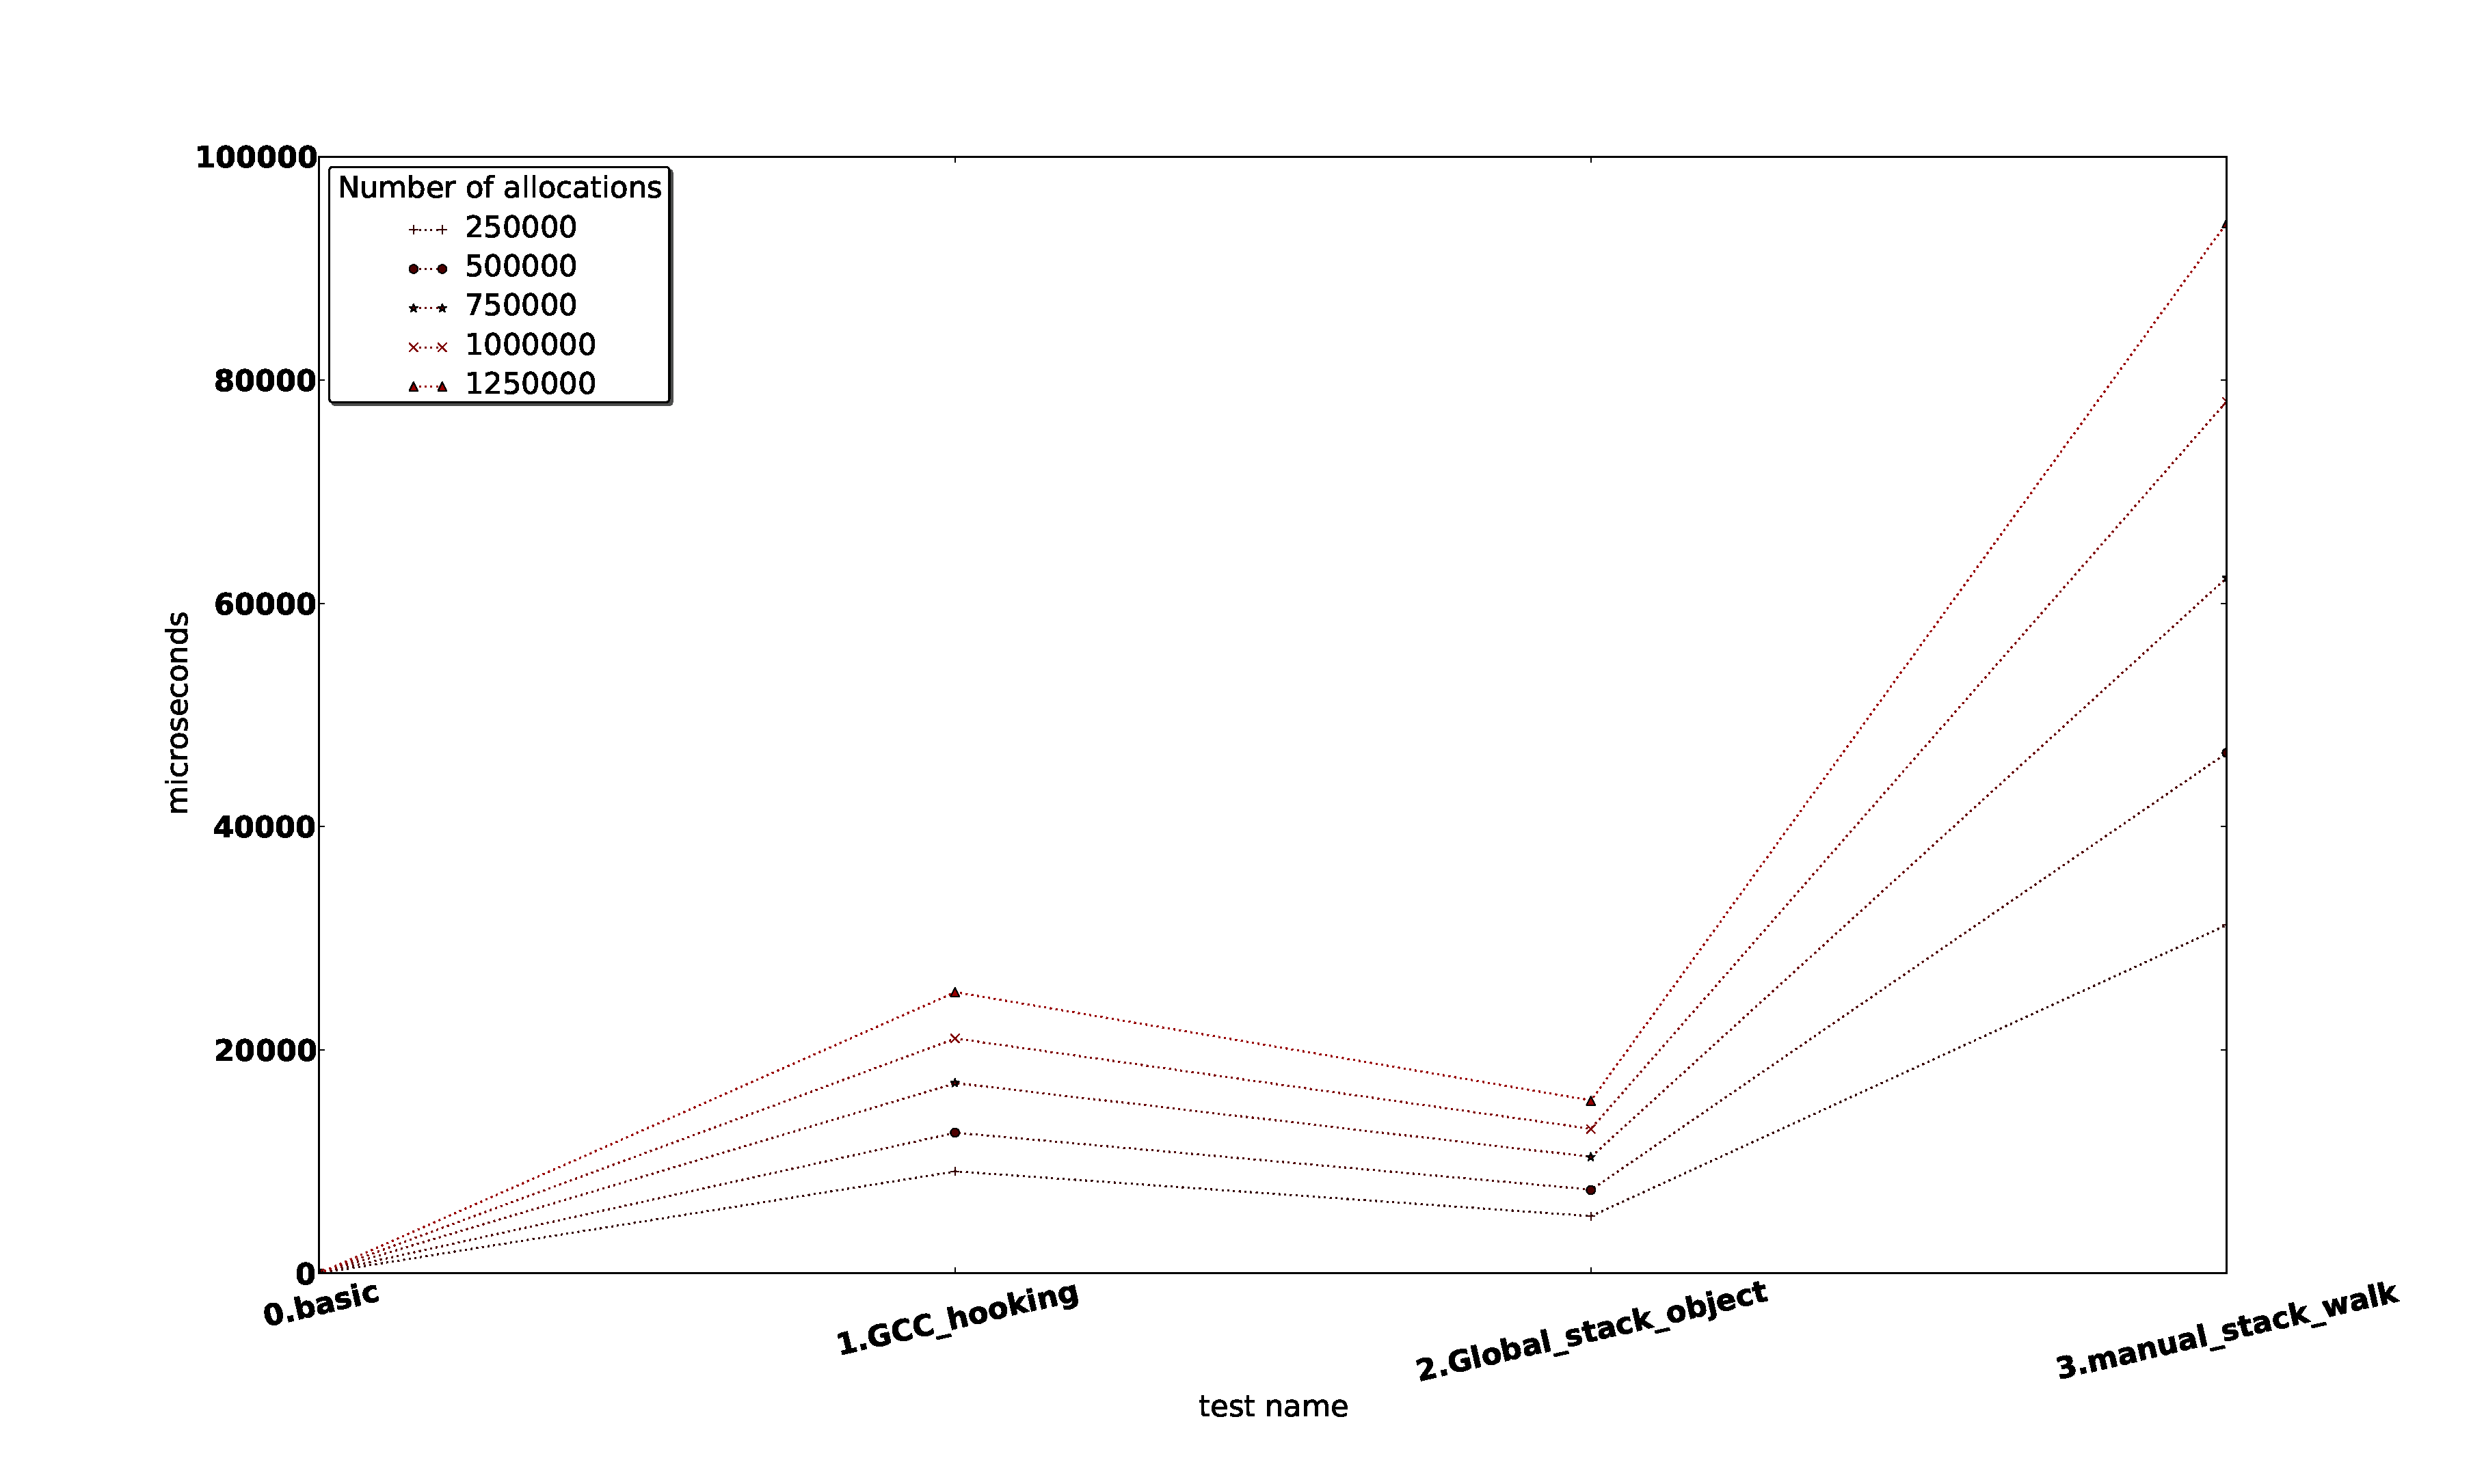
\includegraphics[scale=0.5, width=\textwidth]{src/img/allocationpoint}
\caption{Allocation point time overhead compared to the basic scenario}
\label{fig:allocpoint}
\end{figure}

All of the above methods have some overhead, so the question is if we can minimize that overhead no matter what method we choose. The first observation we can make is that in the method analysis we have tried to obtain stack traces at each and every allocation the program makes. While this does provide a complete view of an application's memory usage characteristics it is unnecessary for analysis targeting memory spikes and high memory consumption, which is what we are interested in. The typical usage scenario of the profiler we want is the following:

\begin{enumerate}
\item Have a complete view of the memory consumption of different modules in the application
\item Observe one or more modules which show an unusually high memory consumption
\item Trigger more in-depth analysis of those modules by showing the most frequently called allocations done inside the module
\item Enable stack trace logging only for those allocations which are frequently called
\end{enumerate}

By doing the above we can see the call chain which leads to frequent allocations and identify points which can be optimized for better performance.

This is the part where the low-overhead tracepoints come into play. Each allocation routine can have such a tracepoint attached which is disabled by default, by being a noop. The tracepoint, when enabled, does a jump to a routine which either does a simple call count or a full-fledged stack trace, depending on a flag. The enabling of these tracepoints is done entirely on-demand, thus avoiding the overhead of having all the allocation routines do stack trace logging. Combining the tracepoints with any of the allocation point methods above, leads to a lightweight solution that is, however, platform specific and not easily implementable.

\section{Other issues}
\label{section:otherissues}

There are other issues which the tests do not tackle, yet they are for a complete solution:
\begin{enumerate}
\item \textit{Information storage and analysis} - The test programs use a circular, fixed size buffer for storing the stack traces up to a certain depth. This solution has to be extended to add allocation size information and to allow grouping of stack traces. Two allocations made from the same point have the same stack trace and thus the size should be modified accordingly. Exactly how much of the stack trace is to be compared for equality is another discussion. A shallow comparison of just a couple of stack frames from the trace might not be too useful if the allocations are done in a number of function calls larger than the analysis depth. A specialized allocator might be such an implementation and a shallow analysis would just reveal how the allocator works when in fact we are interested in determining who called the allocator. Another related problem is where this analysis should be performed.
\item \textit{Concurrency} - Each thread has its own stack
\end{enumerate}

